\documentclass[11pt,handout]{beamer}

\usepackage{tcolorbox}

% bibliography
\usepackage[backend=biber]{biblatex}
\bibliography{scg_seminar.bib}

\usepackage[cache=false]{minted}
\usepackage{sourcecodepro}

\usepackage{fancyvrb}

% isabelle
\newminted{isabelle}{
  frame=single,
  framesep=2mm,
  fontsize=\scriptsize,
  mathescape
}

\newminted{prolog}{
  frame=single,
  framesep=2mm,
  fontsize=\scriptsize,
  mathescape
}

\newminted{bc}{
  frame=single,
  framesep=2mm,
  fontsize=\scriptsize,
  mathescape
}

\newminted{scala}{
  frame=single,
  framesep=2mm,
  fontsize=\scriptsize,
  mathescape
}

\newminted{java}{
  frame=single,
  framesep=2mm,
  fontsize=\scriptsize,
  mathescape
}


\makeatletter
\AtBeginEnvironment{minted}{\dontdofcolorbox}
\def\dontdofcolorbox{\renewcommand\fcolorbox[4][]{##4}}
\makeatother

\usepackage{graphicx}
\usepackage{amsmath}
\usepackage{bussproofs}
\usepackage{mathpartir}
\usepackage{prooftrees}
\usepackage{color}

% remove the Figure :
\usepackage{caption}
\captionsetup{figurename=}

\usepackage{algorithmicx}
\usepackage{algpseudocode}

\setbeamerfont{footnote}{size=\tiny}

\graphicspath{{img/}}

\usetheme{CambridgeUS}

\author[Sylvain Julmy]{Author : Sylvain Julmy\\\vspace*{0.2cm}Supervisors : Boris Spasojević, Manuel Leuenberger}
\title[SCG Seminar]{Bc running on Truffle}
\date{\today}

\AtBeginSection[]
{
  \begin{frame}
    \frametitle{Table of Contents}
    \tableofcontents[currentsection]
  \end{frame}
}

\begin{document}

\maketitle

\begin{frame}[fragile]
  \frametitle{Project statement}
  
  The goal of this project is to implement \textbf{bc} as a Truffle languages to serve
  the purpose as a simple language to introduce Truffle and improving bc's
  performance.
\end{frame}

\begin{frame}[fragile]
  \frametitle{bc}
  bc (\textbf{b}asic \textbf{c}alculator) is a language that support arbitrary
  precision number and a syntax close to the C programming language.

\begin{bccode}
sum = ( 8866128975287528 ^ 3) +\
      (-8778405442862239 ^ 3) +\
      (-2736111468807040 ^ 3)
print sum, "\n"
halt
\end{bccode}
\end{frame}

\section[GraalVM and Truffle]{GraalVM and Truffle}

\begin{frame}[fragile]
  \frametitle{GraalVM}
  GraalVM is a universal virtual machine for running applications written in
  various languages\footnote{\url{https://www.graalvm.org/}}.

  It aims to :
  \begin{itemize}
  \item match performance of JVM languages with native languages.
  \item allow freeform mixing of programming languages (polyglot applications).
  \item include a set of ``polyglot programming tools''.
  \end{itemize}
\end{frame}

\begin{frame}[fragile]
  \frametitle{Truffle}
  Truffle is a framework for building programming languages as interpreters for
  self-modifying AST.
\end{frame}

\begin{frame}[c,fragile]
  \frametitle{AST Interpreter}

  \begin{minipage}[t]{0.48\textwidth}
\begin{javacode}
class MulNode extends Node {
  Node left;
  Node right;
  int execute() {
    return left.execute() *
           right.execute();
  }
}
\end{javacode}

    Each node compute his own operation.
    
  \end{minipage}
  \hfill
  \begin{minipage}[t]{0.48\textwidth}
  \begin{figure}[ht]
    \centering
    \fbox{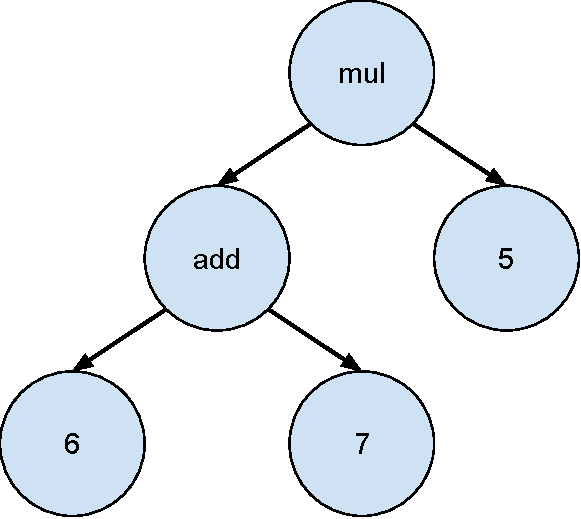
\includegraphics[width=0.99\textwidth]{img/ast-interpreter.pdf}}
    \caption{Simple AST}
    \label{fig:ast-interpreter}
  \end{figure}
  \end{minipage}
\end{frame}

% \begin{frame}[fragile]
%   \frametitle{Node specialization}
%     \begin{figure}[ht]
%     \centering
%     \fbox{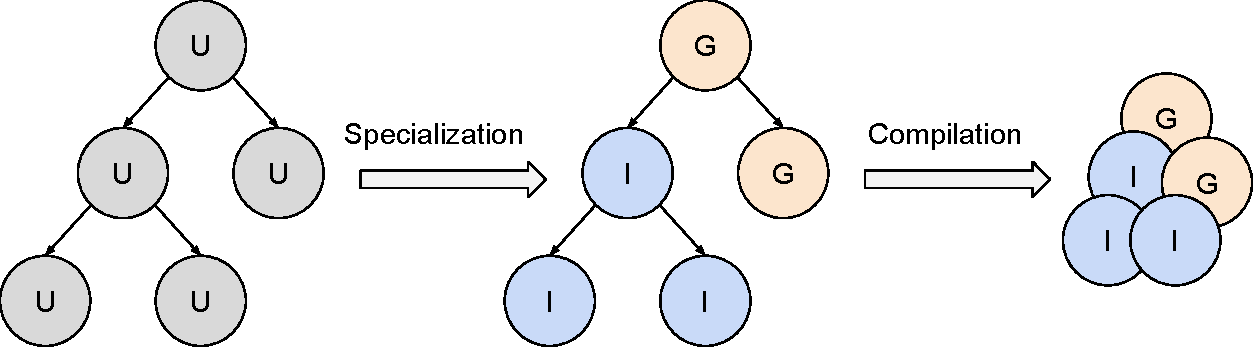
\includegraphics[width=0.99\textwidth]{img/node-specialization.pdf}}
%     \caption{Node specialization}
%     \label{fig:ast-interpreter}
%   \end{figure}
% \end{frame}

% \begin{frame}[fragile]
%   \frametitle{Node specialization}
%     \begin{figure}[ht]
%     \centering
%     \fbox{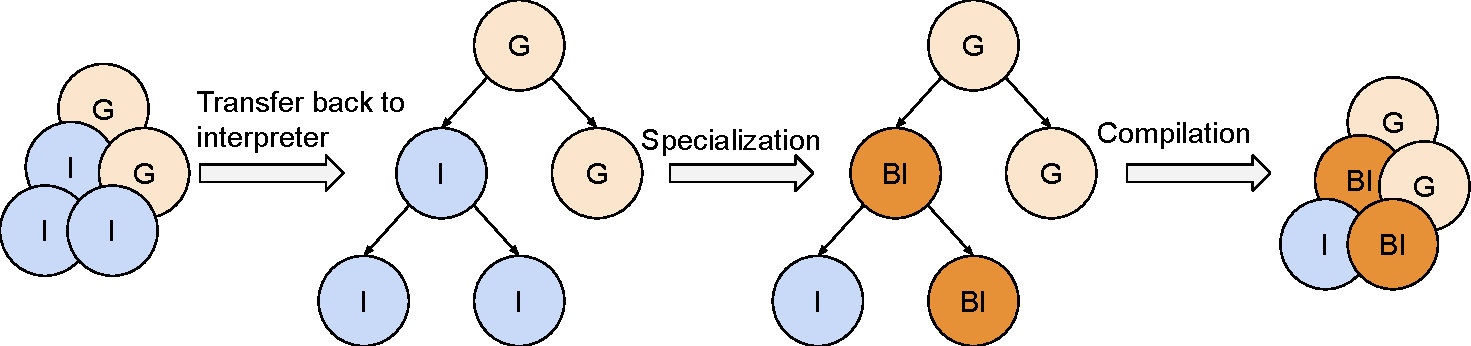
\includegraphics[width=0.99\textwidth]{img/node-recompilation.pdf}}
%     \caption{Node recompilation}
%     \label{fig:ast-interpreter}
%   \end{figure}
% \end{frame}


% \begin{frame}[fragile]
%   \frametitle{Partial evaluation}
%   \[
%     prog : I_{static} \times I_{dynamic} \mapsto O
%   \]

%   Idea of partial evaluation : turning $prog$ into $prog^*$ :

%   \[
%     prog* : I_{dynamic} \mapsto O
%   \]
% \end{frame}

\section[Implementing bc with Truffle]{Implementing bc with Truffle}

\begin{frame}[fragile]
  \frametitle{Global architecture}
  \begin{figure}[ht]
    \centering
    \fbox{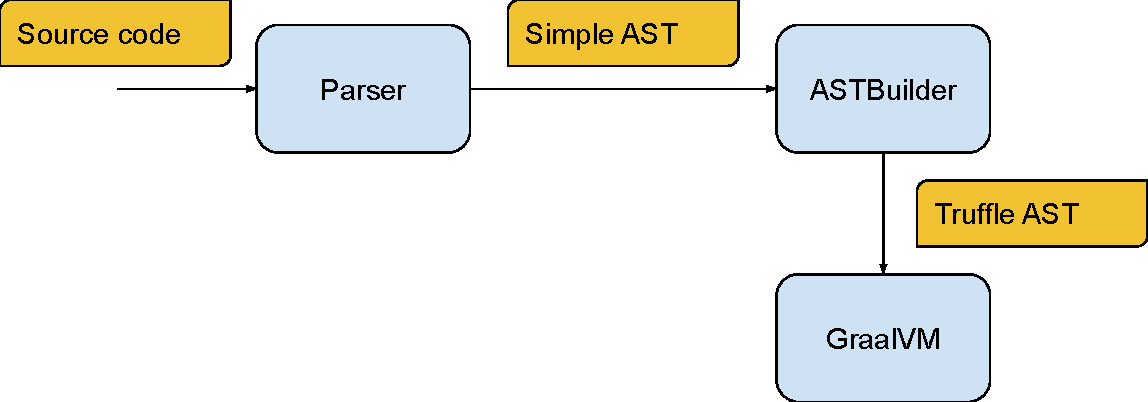
\includegraphics[width=0.9\textwidth]{img/bc-truffle-arch.pdf}}
    \caption{bc-truffle architecture.}
    \label{fig:bc-truffle-arch}
  \end{figure}
\end{frame}

\begin{frame}[fragile]
  \frametitle{Parser}
  Parser is implemented in Scala using parser-combinator and produce an
  intermediate AST.

  The AST is then visited to produce the Truffle AST.
\end{frame}

\begin{frame}[fragile]
  \frametitle{Example : Add node}
\begin{scalacode}
@NodeChildren({
        @NodeChild(value = "left", type = BcExpressionNode.class),
        @NodeChild(value = "right", type = BcExpressionNode.class)
})
public abstract class BcBinaryNode extends BcExpressionNode {}
\end{scalacode}
\end{frame}

\begin{frame}[fragile]
  \frametitle{Example : Add node}
\begin{scalacode}
  public abstract class BcAddNode extends BcBinaryNode {

    @Specialization(rewriteOn = ArithmeticException.class)
    protected long add(long left, long right) {
        return Math.addExact(left, right);
    }

    @Specialization
    protected BcBigNumber add(BcBigNumber left, BcBigNumber right) {
      return left.add(right);
    }

    @Specialization
    protected String doString(Object left, Object right) {
      return left.toString() + right.toString();
    }

    @Fallback
    protected Object typeError(Object left, Object right) {
      throw BcException.typeError(this, left, right);
    }
  }
\end{scalacode}
\end{frame}

\section[Performance]{Performance}

\begin{frame}[fragile]
  \frametitle{bc-truffle vs. Java vs. bc}
  Here is a simple program which multiply big number :

  \begin{minipage}[t]{0.64\textwidth}
\begin{javacode}
import java.math.BigDecimal;
class Bignumber {
  public static void main(String[] args) {
    BigDecimal y = new BigDecimal(1);
    for(int i=1; i<500_000;i++) {
      y = y.multiply(new BigDecimal(i));
    }
    System.out.println(y);
  }
}
\end{javacode}
  \end{minipage}
  \hfill
  \begin{minipage}[t]{0.35\textwidth}
\begin{bccode}
  y = 1
  for(i=1;i<500000;i++)
    y *= i
  y
  halt
\end{bccode}
  \end{minipage}
  
  \begin{center}
  Java time  : 103s  \\
  bc-truffle : 105s  \\
  bc         : 4213s \\
  \end{center}
\end{frame}

\begin{frame}[fragile]
  \frametitle{bc-truffle vs. Java vs. bc}
    \begin{figure}[ht]
    \centering
    \fbox{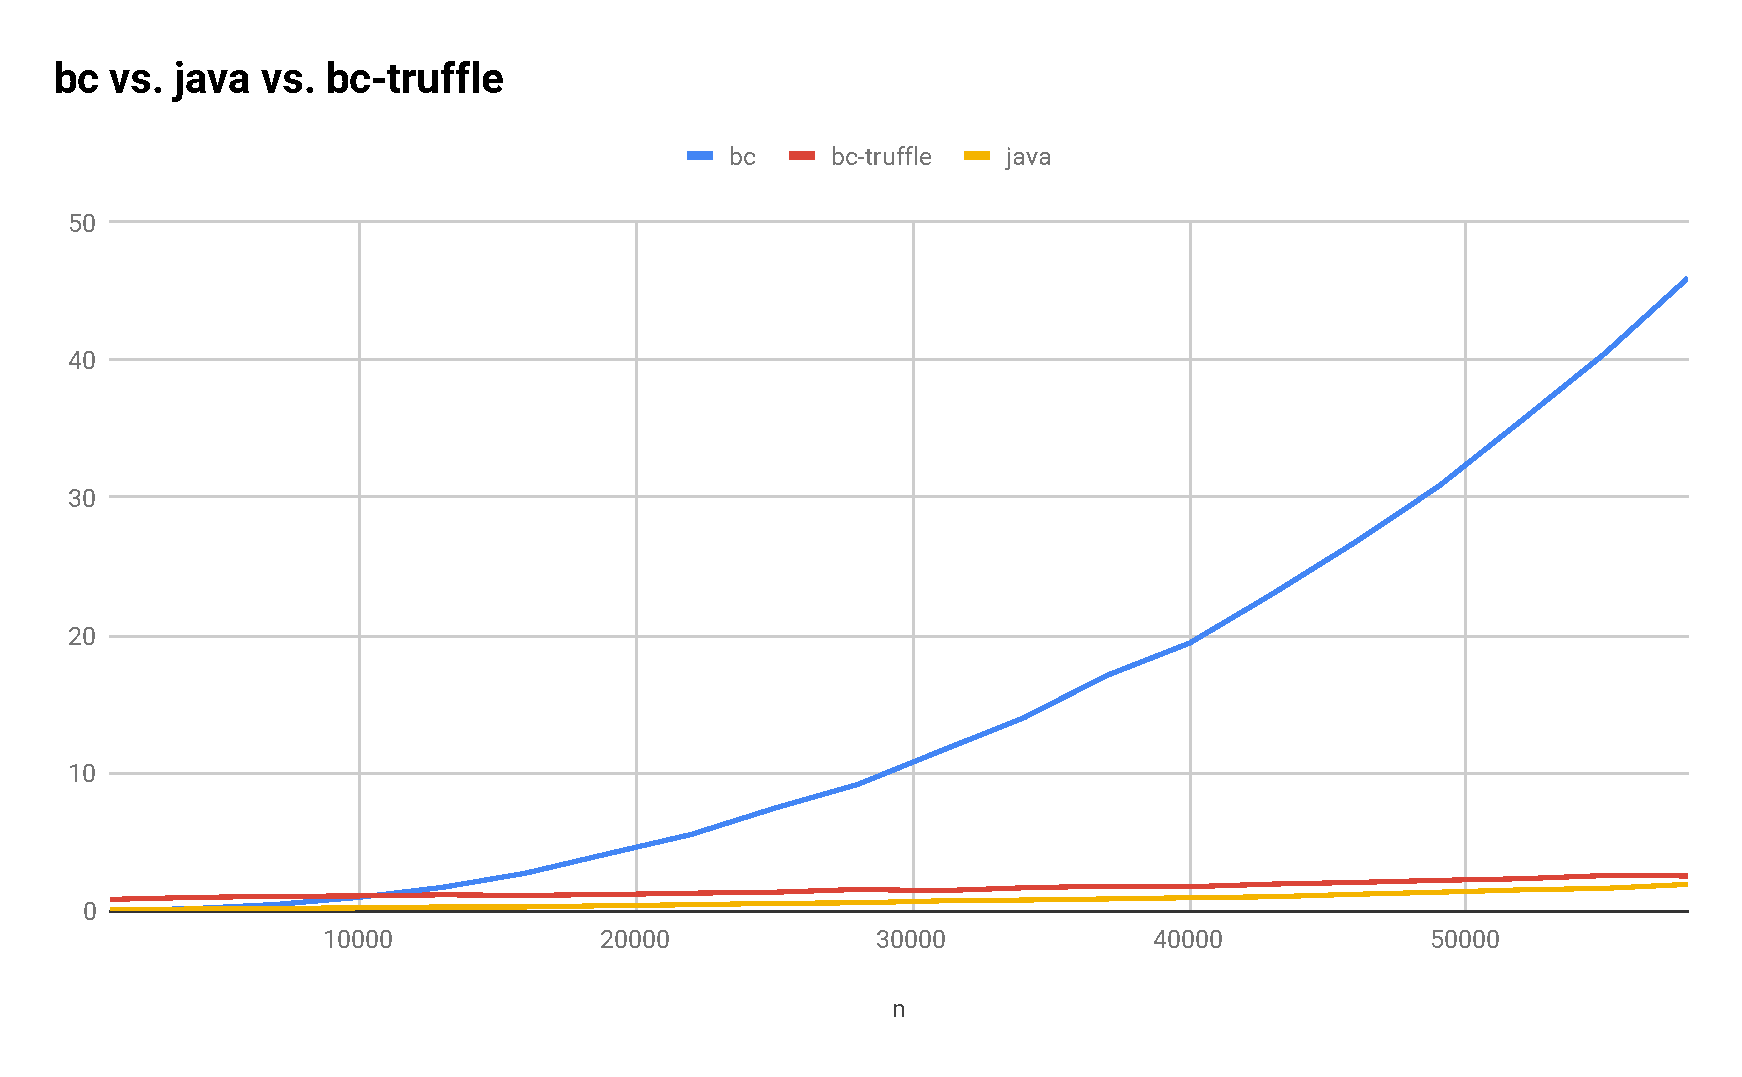
\includegraphics[width=0.9\textwidth]{img/bc_comp_3.pdf}}
    \caption{bc-truffle vs. Java vs. bc}
    \label{fig:comp_3}
  \end{figure}
\end{frame}

\begin{frame}[fragile]
  \frametitle{bc-truffle vs. Java}
    \begin{figure}[ht]
    \centering
    \fbox{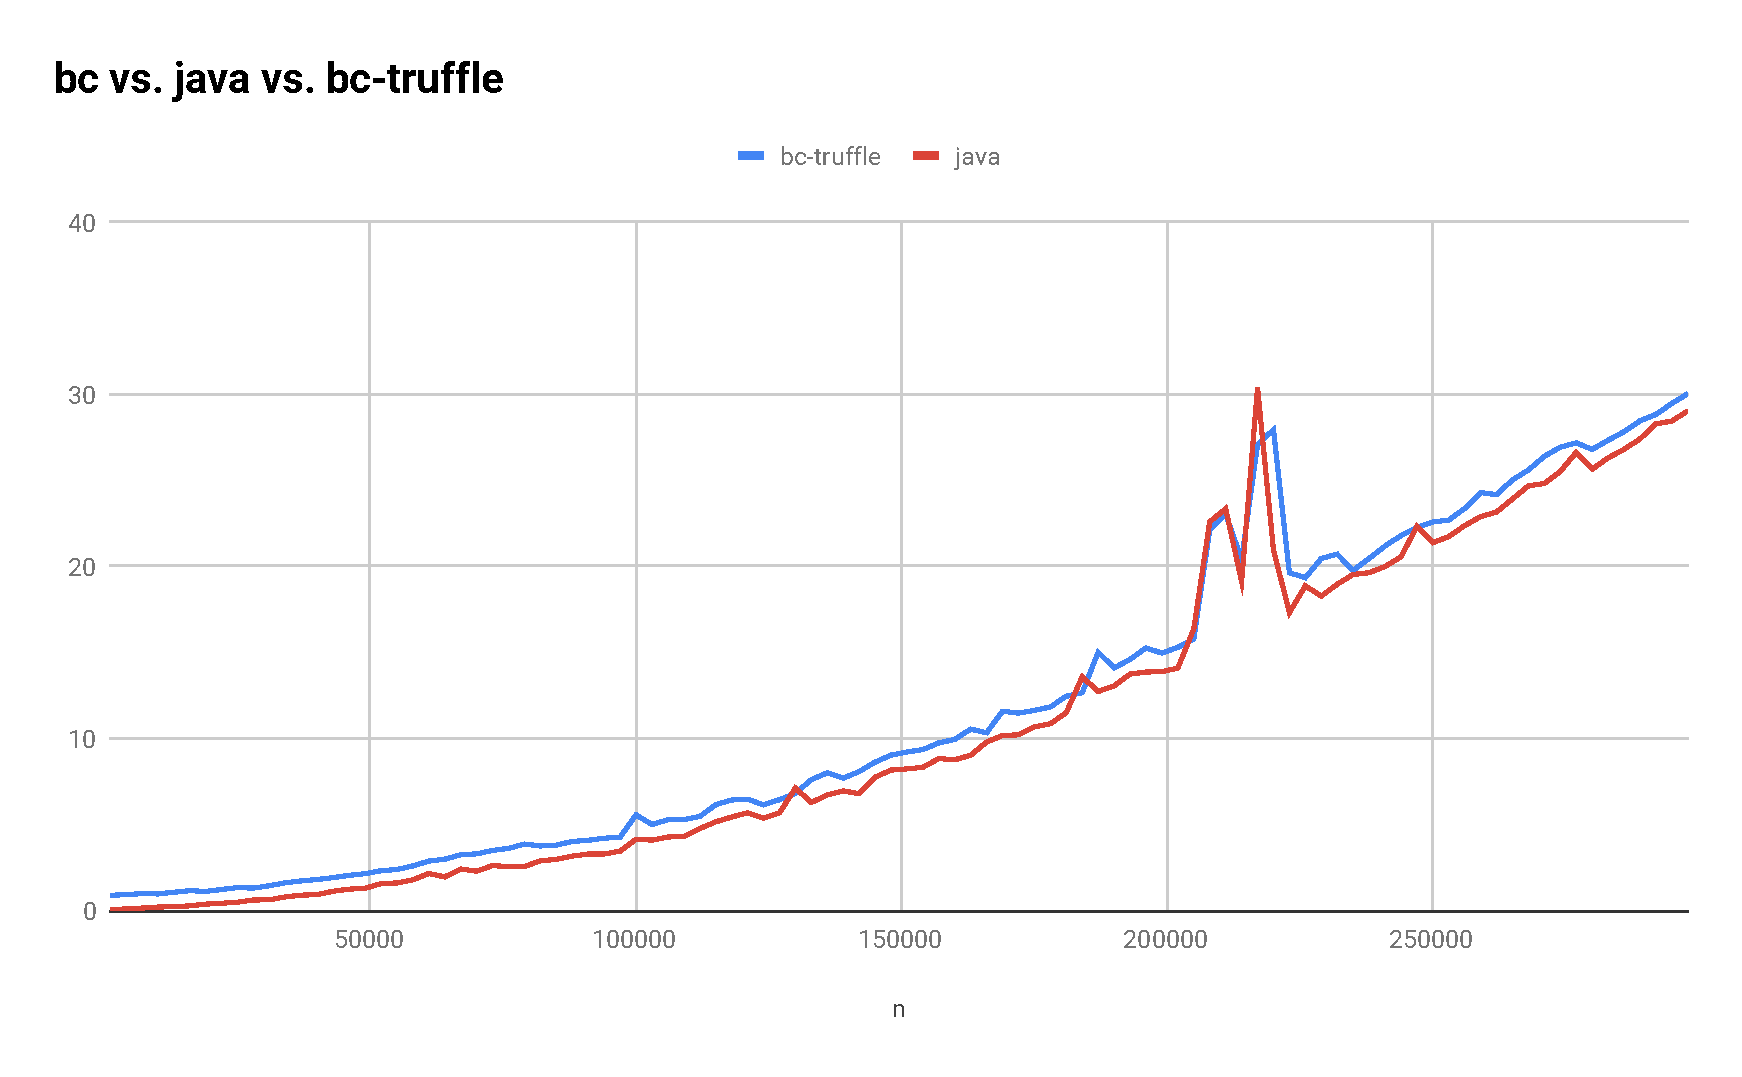
\includegraphics[width=0.9\textwidth]{img/bc_comp_2.pdf}}
    \caption{bc-truffle vs. Java vs. bc}
    \label{fig:comp_2}
  \end{figure}
\end{frame}

\begin{frame}[fragile]
  \frametitle{Native image}
  The native image allows to ahead-of-time compile Java code to a standalone
  executable.
\end{frame}

\section[Conclusion]{Conclusion}

\begin{frame}[fragile]
  \frametitle{Using Truffle}
  \begin{itemize}
  \item Simple language is a good introduction to understand some basic concept.
  \item Read some Truffle paper.
  \item Blog post about implementing a Lisp.
  \item Look at the others implementation.
  \end{itemize}
\end{frame}

\begin{frame}[fragile]
  \frametitle{Improvement}
  \begin{itemize}
  \item Support all the bc's extensions (i.e. GNU bc).
  \item Add tool support.
  \item Add more opportunity for optimization.
  \item Support interoperability for polyglot applications.
  \item Find and fix bugs !
  \end{itemize}
\end{frame}

\begin{frame}[fragile]
  \frametitle{Links}
  Github repository :

  \url{https://github.com/SnipyJulmy/bc-truffle}
\end{frame}

% \begin{frame}
% \frametitle{References}
% \printbibliography
% \end{frame}

\end{document}